\qrchapterstar{https://forgottenpillar.com/rsc/en-fp-appendix}{Appendix} \label{chap:appendix}

\addcontentsline{toc}{chapter}{Appendix}

\section*{The Fundamental Principles 1889}

As elsewhere stated, Seventh-day Adventists have no creed but the Bible; but they hold to certain well-defined points of faith for which they feel prepared to give a reason “to every man that asketh” them. The following propositions may be taken as a summary of the principal features of their religious faith, upon which there is, so far as we know, entire unanimity throughout the body. They believe,— 

\lettrine{I.} That there is one God, a personal, spiritual being, the creator of all things, omnipotent, omniscient, and eternal; infinite in wisdom, holiness, justice, goodness, truth, and mercy; unchangeable, and everywhere present by his representative, the Holy Spirit. Psalm 139:7.

\lettrine{II.} That there is one Lord Jesus Christ, the Son of the Eternal Father, the one by whom he created all things, and by whom they do consist; that he took on him the nature of the seed of Abraham for the redemption of our fallen race; that he dwelt among men, full of grace and truth, lived our example, died our sacrifice, was raised for our justification, ascended on high to be our only mediator in the sanctuary in heaven, where, through the merits of his shed blood, he secures the pardon and forgiveness of the sins of all those who penitently come to him; and as the closing portion of his work as priest, before he takes his throne as king, he will make the great atonement for the sins of all such, and their sins will then be blotted out (Acts 3:19) and borne away from the sanctuary, as shown in the service of the Levitical priesthood, which foreshadowed and prefigured the ministry of our Lord in heaven. See Leviticus 16; Hebrews 8:4, 5; 9:6, 7; etc.

\lettrine{III.} That the Holy Scriptures of the Old and New Testaments were given by inspiration of God, contain a full revelation of his will to man, and are the only infallible rule of faith and practice.

\lettrine{IV.} That baptism is an ordinance of the Christian church, to follow faith and repentance,—an ordinance by which we commemorate the resurrection of Christ, as by this act we show our faith in his burial and resurrection, and through that, in the resurrection of all the saints at the last day; and that no other mode more fitly represents these facts than that which the Scriptures prescribe, namely, immersion. Romans 6:3-5; Colossians 2:12.

\lettrine{V.} That the new birth comprises the entire change necessary to fit us for the kingdom of God, and consists of two parts; First, a moral change wrought by conversion and a Christian life (John 3:3, 5); second, a physical change at the second coming of Christ, whereby, if dead, we are raised incorruptible, and if living, are changed to immortality in a moment, in the twinkling of an eye. Luke 20:36; 1 Corinthians 15:51, 52.

\lettrine{VI.} That prophecy is a part of God’s revelation to man; that it is included in that Scripture which is profitable for instruction (2 Timothy 3:16); that it is designed for us and our children (Deuteronomy 29:29); that so far from being enshrouded in impenetrable mystery, it is that which especially constitutes the word of God a lamp to our feet and a light to our path (Psalm 119:105; 2 Peter 1:19); that a blessing is pronounced upon those who study it (Revelation 1:1-3); and that, consequently, it is to be understood by the people of God sufficiently to show them their position in the world’s history and the special duties required at their hands.

\lettrine{VII.} That the world’s history from specified dates in the past, the rise and fall of empires, and the chronological succession of events down to the setting up of God’s everlasting kingdom, are outlined in numerous great chains of prophecy; and that these prophecies are now all fulfilled except the closing scenes.

\lettrine{VIII.} That the doctrine of the world’s conversion and a temporal millennium is a fable of these last days, calculated to lull men into a state of carnal security, and cause them to be overtaken by the great day of the Lord as by a thief in the night (1 Thessalonians 5:3); that the second coming of Christ is to precede, not follow, the millennium; for until the Lord appears, the papal power, with all its abominations, is to continue (2 Thessalonians 2:8), the wheat and tares grow together (Matthew 13:29, 30, 39), and evil men and seducers wax worse and worse, as the word of God declares. 2 Timothy 3:1, 13.

\lettrine{IX.} That the mistake of Adventists in 1844 pertained to the nature of the event then to transpire, not to the time; that no prophetic period is given to reach to the second advent, but that the longest one, the two thousand and three hundred days of Daniel 8:14, terminated in 1844, and brought us to an event called the cleansing of the sanctuary.

\lettrine{X.} That the sanctuary of the new covenant is the tabernacle of God in heaven, of which Paul speaks in Hebrews 8 and onward, and of which our Lord, as great high priest, is minister; that this sanctuary is the antitype of the Mosaic tabernacle, and that the priestly work of our Lord, connected therewith, is the antitype of the work of the Jewish priests of the former dispensation (Hebrews 8:1-5, etc.); that this, and not the earth, is the sanctuary to be cleansed at the end of the two thousand and three hundred days, what is termed its cleansing being in this case, as in the type, simply the entrance of the high priest into the most holy place, to finish the round of service connected therewith, by making the atonement and removing from the sanctuary the sins which had been transferred to it by means of the ministration in the first apartment (Leviticus 16; Hebrews 9:22, 23); and that this work in the antitype, beginning in 1844, consists in actually blotting out the sins of believers (Acts 3:19), and occupies a brief but indefinite space of time, at the conclusion of which the work of mercy for the world will be finished, and the second advent of Christ will take place.

\lettrine{XI.} That God’s moral requirements are the same upon all men in all dispensations; that these are summarily contained in the commandments spoken by Jehovah from Sinai, engraven on the tables of stone, and deposited in the ark, which was in consequence called the “ark of the covenant,” or testament (Numbers 10:33; Hebrews 9:4, etc.); that this law is immutable and perpetual, being a transcript of the tables deposited in the ark in the true sanctuary on high, which is also, for the same reason, called the ark of God’s testament; for under the sounding of the seventh trumpet we are told that “the temple of God was opened in heaven, and there was seen in his temple the ark of his testament.” Revelation 11:19. 

\lettrine{XII.} That the fourth commandment of this law requires that we devote the seventh day of each week, commonly called Saturday, to abstinence from our own labor, and to the performance of sacred and religious duties; that this is the only weekly Sabbath known to the Bible, being the day that was set apart before Paradise was lost (Genesis 2:2, 3), and which will be observed in Paradise restored (Isaiah 66:22, 23); that the facts upon which the Sabbath institution is based confine it to the seventh day, as they are not true of any other day; and that the terms Jewish Sabbath, as applied to the seventh day, and Christian Sabbath, as applied to the first day of the week, are names of human invention, unscriptural in fact, and false in meaning.

\lettrine{XIII.} That as the man of sin, the papacy, has thought to change times and laws (the law of God, Daniel 7:25), and has misled almost all Christendom in regard to the fourth commandment, we find a prophecy of a reform in this respect to be wrought among believers just before the coming of Christ. Isaiah 56:1, 2; 1 Peter 1:5; Revelation 14:12, etc.

\lettrine{XIV.} That the followers of Christ should be a peculiar people, not following the maxims, nor conforming to the ways, of the world; not loving its pleasures nor countenancing its follies; inasmuch as the apostle says that “whosoever therefore will be” in this sense, “a friend of the world, is the enemy of God” (James 4:4); and Christ says that we cannot have two masters, or, at the same time, serve God and mammon. Matthew 6:24.

\lettrine{XV.} That the Scriptures insist upon plainness and modesty of attire as a prominent mark of discipleship in those who profess to be the followers of Him who was, “meek and lowly in heart,” that the wearing of gold, pearls, and costly array, or anything designed merely to adorn the person and foster the pride of the natural heart, is to be discarded, according to such scriptures as 1 Timothy 2:9, 10; 1 Peter 3:3, 4.

\lettrine{XVI.} That means for the support of evangelical work among men should be contributed from love to God and love of souls, not raised by church lotteries, or occasions designed to contribute to the fun-loving, appetite-indulging propensities of the sinner, such as fairs, festivals, oyster suppers, tea, broom, donkey, and crazy socials, etc., which are a disgrace to the professed church of Christ; that the proportion of one’s income required in former dispensation can be no less under the gospel; that it is the same as Abraham (whose children we are, if we are Christ’s, Galatians 3:29) paid to Melchisedec (type of Christ) when he gave him a tenth of all (Hebrews 7:1-4); the title is the Lord’s (Leviticus 27:30); and this tenth of one’s income is also to be supplemented by offerings from those who are able, for the support of the gospel. 2 Corinthians 9:6; Malachi 3:8, 10.

\lettrine{XVII.} That as the natural or carnal heart is at enmity with God and his law, this enmity can be subdued only by a radical transformation of the affections, the exchange of unholy for holy principles; that this transformation follows repentance and faith, is the special work of the Holy Spirit, and constitutes regeneration, or conversion.

\lettrine{XVIII.} That as all have violated the law of God, and cannot of themselves render obedience to his just requirements, we are dependent on Christ, first, for justification from our past offenses, and, secondly, for grace whereby to render acceptable obedience to his holy law in time to come.

\lettrine{XIX.} That the Spirit of God was promised to manifest itself in the church through certain gifts, enumerated especially in 1 Corinthians 12 and Ephesians 4; that these gifts are not designed to supersede, or take the place of, the Bible, which is sufficient to make us wise unto salvation, any more than the Bible can take the place of the Holy Spirit; that, in specifying the various channels of its operation, that Spirit has simply made provision for its own existence and presence with the people of God to the end of time, to lead to an understanding of that word which it had inspired, to convince of sin, and to work a transformation in the heart and life; and that those who deny to the Spirit its place and operation, do plainly deny that part of the Bible which assigns to it this work and position.

\lettrine{XX.} That God, in accordance with his uniform dealings with the race, sends forth a proclamation of the approach of the second advent of Christ; and that this work is symbolized by the three messages of Revelation 14, the last one bringing to view the work of reform on the law of God, that his people may acquire a complete readiness for that event.

\lettrine{XXI.} That the time of the cleansing of the sanctuary (See proposition X.), synchronizing with the time of the proclamation of the third message (Revelation 14:9, 10), is a time of investigative judgment, first, with reference to the dead, and secondly, at the close of probation, with reference to the living, to determine who of the myriads now sleeping in the dust of the earth are worthy of a part in the first resurrection, and who of its living multitudes are worthy of translation,—points which must be determined before the Lord appears.

\lettrine{XXII.} That the grave, whether we all tend, expressed by the Hebrew word sheol and the Greek word hades, is a place, or condition, in which there is no work, device, wisdom, nor knowledge. Ecclesiastes 9:10.

\lettrine{XXIII.} That the state to which we are reduced by death is one of silence, inactivity, and entire unconsciousness. Psalm 146:4; Ecclesiastes 9:5, 6; Daniel 12:2.

\lettrine{XXIV.} That out of this prison-house of the grave, mankind are to be brought by a bodily resurrection; the righteous having part in the first resurrection, which takes place at the second coming of Christ; the wicked, in the second resurrection, which takes place in a thousand years thereafter. Revelation 20:4-6.

\lettrine{XXV.} That at the last trump, the living righteous are to be changed in a moment, in the twinkling of an eye, and with the risen righteous are to be caught up to meet the Lord in the air, so forever to be with the Lord. 1 Thessalonians 4:16, 17; 1 Corinthians 15:51, 52.

\lettrine{XXVI.} That these immortalized ones are then taken to heaven, to the New Jerusalem, the Father’s house, in which there are many mansions (John 14:1-3), where they reign with Christ a thousand years, judging the world and fallen angels, that is, apportioning the punishment to be executed upon them at the close of the one thousand years (Revelation 20:4; 1 Corinthians 6:2, 3); that during this time the earth lies in a desolate and chaotic condition (Jeremiah 4:23-27), described, as in the beginning, by the Greek term abussos— “bottom-less pit” (Septuagint of Genesis 1:2); and that here Satan is confined during the thousand years (Revelation 20:1, 2), and here finally destroyed (Revelation 20:10; Malachi 4:1); the theater of the ruin he has wrought in the universe being appropriately made, for a time, his gloomy prison-house, and then the place of his final execution.

\lettrine{XXVII.} That at the end of the thousand years the Lord descends with his people and the New Jerusalem (Revelation 21:2), the wicked dead are raised, and come up on the surface of the yet unrenewed earth, and gather about the city, the camp of the saints (Revelation 20:9), and fire comes down from God out of heaven and devours them. They are then consumed, root and branch (Malachi 4:1), becoming as though they had not been. Obadiah 15, 16. In this everlasting destruction from the presence of the Lord (2 Thessalonians 1:9), the wicked meet the “everlasting punishment” threatened against them (Matthew 25:46), which is everlasting death. Romans 6:23; Revelation 20:14, 15. This is the perdition of ungodly men, the fire which consumes them being the fire for which “the heavens and the earth, which are now,... are kept in store.” which shall melt even the elements with its intensity, and purge the earth from the deepest stains of the curse of sin. 2 Peter 3:7-12.

\lettrine{XXVIII.} That new heavens and a new earth shall spring by the power of God from the ashes of the old, and this renewed earth, with the New Jerusalem for its metropolis and capital, shall be the eternal inheritance of the saints, the place where the righteous shall evermore dwell. 2 Peter 3:13; Psalm 37:11, 29; Matthew 5:5. 



\section*{Fundamental Principles - Timeline} \label{appendix:timeline}

The following is a list of some appearances of the Declaration of Fundamental Principles in our publications. All links are accessible at \href{https://notefp.link/fp-timeline}{https://notefp.link/fp-timeline}.

\leftsubsection{1872 - The first appearance}

\textit{“A Declaration of the Fundamental Principles Taught and Practiced by Seventh-day Adventists}” - printed as a pamphlet (\href{https://adventistdigitallibrary.org/islandora/object/adl:366607?link_only=true}{original scan} \href{https://forgotten-pillar.s3.us-east-2.amazonaws.com/A+declaration+of+the+fundamental+principles+taught+and+practiced+by+the+Seventh-day+Adventists++.pdf}{*}). They appeared anonymous, presented as a short public synopsis of what Seventh-day Adventists believe.

\leftsubsection{1874 - The Signs of the Times}

Original scan: \href{https://adventistdigitallibrary.org/adl-364148/signs-times-june-4-1874}{ST June 4, 1874, p.3.} \href{https://forgotten-pillar.s3.us-east-2.amazonaws.com/Signs+of+the+Times+_+June+4%2C+1874++.pdf}{*} James White stood behind the declaration as a main editor of the Signs of the Times at that time.

\leftsubsection{1874 - The Advent Review and Herald of the Sabbath}

Original scan: \href{https://documents.adventistarchives.org/Periodicals/RH/RH18741124-V44-22.pdf}{RH November 24, 1874, p.171} \href{https://forgotten-pillar.s3.us-east-2.amazonaws.com/RH18741124-V44-22.pdf}{*} Uriah Smith signed the declaration as the main editor of the Review and Herald of the Sabbath periodical at that time.

\leftsubsection{1874 - Part of a booklet: The Seventh-day Adventists: A Brief Sketch of Their Origin, Progress, and Principles}

Booklet was reprinted in 1876 and 1878 and later years. \\
Original scan: (\href{https://adventistdigitallibrary.org/islandora/object/adl%3A22250872?solr_nav%5Bid%5D=a09d3902c2540c98eb7f&solr_nav%5Bpage%5D=56&solr_nav%5Boffset%5D=3}{1878 copy})

\leftsubsection{1875 - The Signs of the Times}

Original scan: \href{https://documents.adventistarchives.org/Periodicals/ST/ST18750128-V01-14.pdf#search=ST18750128}{ST January 28, 1875} \href{https://forgotten-pillar.s3.us-east-2.amazonaws.com/ST18750128-V01-14.pdf}{*} (p. 108, 109)

\leftsubsection{1878 - The Signs of the Times}

Original scan: \href{https://documents.adventistarchives.org/Periodicals/ST/ST18780221-V04-08.pdf#search=%22As%20already%20stated%2C%20S%2E%20D%2E%20Adventists%22}{ST February 21, 1878} \href{https://forgotten-pillar.s3.us-east-2.amazonaws.com/ST18780221-V04-08.pdf}{*} (p. 59)

\leftsubsection{1888 - Gospel Sickle, April 1, 1888}

Original scan: \href{https://adventistdigitallibrary.org/adl-410336/gospel-sickle-april-1-1888?view_only=true&solr_nav%5Bid%5D=ff4d7f3f77b9bdf9e9ac&solr_nav%5Bpage%5D=0&solr_nav%5Boffset%5D=6}{Gospel Sickle, April 1, 1888}

\leftsubsection{1888 - The Present Truth, August 16, 1888}

Original scan: \href{https://adventistdigitallibrary.org/adl-402854/present-truth-august-16-1888?view_only=true&solr_nav%5Bid%5D=ff4d7f3f77b9bdf9e9ac&solr_nav%5Bpage%5D=0&solr_nav%5Boffset%5D=13}{PT18880816} (p. 250 - 252)

\leftsubsection{1889 - SDA Yearbook for 1889}

Original scan: \href{https://documents.adventistarchives.org/Yearbooks/YB1889.pdf#search=Yearbook%201889}{YB1889} \href{https://forgotten-pillar.s3.us-east-2.amazonaws.com/YB1889.pdf}{*} (p. 145 - 151) Uriah Smith extended Fundamental Principles to 28 propositions. He added point on sanctification (point 14), dress reform (point 15) and tithing (point 16). Also he made small textual changes in some expressions, but semantics remained the same.

\leftsubsection{1897 - Words of Truth - no. 5}

Original scan: \href{https://adl.b2.adventistdigitallibrary.org/concern/published_works/4ffda25e-a06b-48d4-8ace-67cdcd33726f}{WoT no.5}
Word of Truth was a series of pamphlets with \href{https://adl.b2.adventistdigitallibrary.org/concern/parent/22267078_fundamental_principles_of_seventh_day_adventists/published_works/94a22141-33e8-4b9a-b397-2fe48c17bec4}{29 sections}.

\leftsubsection{1905 - SDA Yearbook for 1905}

Original scan: \href{https://documents.adventistarchives.org/Yearbooks/YB1905.pdf#search=Yearbook%201905}{YB1905} \href{https://forgotten-pillar.s3.us-east-2.amazonaws.com/YB1905.pdf}{*} (p. 188 - 192)

\leftsubsection{1907 - SDA Yearbook for 1907}

Original scan: \href{https://documents.adventistarchives.org/Yearbooks/YB1907.pdf#search=Yearbook%201906}{YB1907} \href{https://forgotten-pillar.s3.us-east-2.amazonaws.com/YB1907.pdf}{*} (p. 175 - 179)

\leftsubsection{1908 - SDA Yearbook for 1908}

Original scan: \href{https://documents.adventistarchives.org/Yearbooks/YB1908.pdf#search=Yearbook%201906}{YB1908} \href{https://forgotten-pillar.s3.us-east-2.amazonaws.com/YB1908.pdf}{*} (p. 213 - 217)

\leftsubsection{1909 - SDA Yearbook for 1909}

Original scan: \href{https://documents.adventistarchives.org/Yearbooks/YB1909.pdf#search=Yearbook%201909}{YB1909} \href{https://forgotten-pillar.s3.us-east-2.amazonaws.com/YB1909.pdf}{*} (p. 220 - 224)

\leftsubsection{1910 - SDA Yearbook for 1910}

Original scan: \href{https://documents.adventistarchives.org/Yearbooks/YB1910.pdf#search=Yearbook%201910}{YB1910} \textbf{\href{https://forgotten-pillar.s3.us-east-2.amazonaws.com/YB1910.pdf}{*}} (p. 224 - 228)

\leftsubsection{1911 - SDA Yearbook for 1911}

Original scan: \href{https://documents.adventistarchives.org/Yearbooks/YB1911.pdf#search=Yearbook%201910}{YB1911} \href{https://forgotten-pillar.s3.us-east-2.amazonaws.com/YB1911.pdf}{*} (p. 223 - 227)

\leftsubsection{1912 - Advent Review and Sabbath Herald, August 22, 1912}

Original scan: \href{https://adventistdigitallibrary.org/adl-351682/advent-review-and-sabbath-herald-august-22-1912?view_only=true&solr_nav%5Bid%5D=ff4d7f3f77b9bdf9e9ac&solr_nav%5Bpage%5D=0&solr_nav%5Boffset%5D=15}{RH19120822} (p. 4 - 6)

\leftsubsection{1912 - SDA Yearbook for 1912}

Original scan: \href{https://documents.adventistarchives.org/Yearbooks/YB1912.pdf#search=Yearbook%201910}{YB1912} \href{https://forgotten-pillar.s3.us-east-2.amazonaws.com/YB1912.pdf}{*} (p. 261 - 265)

\leftsubsection{1913 - SDA Yearbook for 1913}

Original scan: \href{https://documents.adventistarchives.org/Yearbooks/YB1913.pdf#search=Yearbook%201913}{YB1913} \href{https://forgotten-pillar.s3.us-east-2.amazonaws.com/YB1913.pdf}{*} (p. 281 -285 )

\leftsubsection{1914 - SDA Yearbook for 1914}
Original scan: \href{https://documents.adventistarchives.org/Yearbooks/YB1914.pdf#search=Yearbook%201914}{YB1914} \href{https://forgotten-pillar.s3.us-east-2.amazonaws.com/YB1914.pdf}{*} (p. 293 - 297)

\section*{Unauthenticated reports in Ellen White writings}

\label{appendix:unauthenticated-reports}
We would like to present to you one Ellen White quotation that challenges the conclusion on the personality of the Holy Spirit. In this study, we have seen that the Holy Spirit is a spirit and not a being. In studying the \emcap{personality of God} and where His presence is, we have seen the distinction between the terms ‘being’ and ‘spirit’. We came to the conclusion that the Father and the Son are two distinct beings, thus constrained in space, while the Holy Spirit is a spirit, a means by which the Father and Son are everywhere present.

The following quotation testifies that the Holy Spirit is also a being, just as the Father and Son are:

\egw{Here is where the work of the Holy Ghost comes in, after your baptism. You are baptized in the name of \textbf{the Father, of the Son, and of the Holy Ghost}. You are raised up out of the water to live henceforth in newness of life—to live a new life. You are born unto God, and you stand under the sanction and \textbf{the power of the three holiest \underline{beings} in heaven}, who are able to keep you from falling.}[Ms95-1906.29; 1906][https://egwwritings.org/read?panels=p8872.35]

Many have come across this quotation and presented it as proof that the Holy Spirit is a being rather than a spirit. In the following, we present our concerns.

The source of this quotation is Manuscript 95, 1906. 

This quotation is actually a report from the sermon Sister White held in Oakland, California, on Sabbath afternoon, October 20, 1906. Many of Ellen White’s public sermons were stenographically reported and later rewritten for publication. When Sister White preached, she never had a written sermon. There were no tape recorders at that time that could accurately document word for word. The only reference we have from that time is the report by the stenographer. This opens the possibility for human error in reporting, or later editing, prior to publication. The plethora of evidence presented in this book makes it clear that this statement is not in harmony with the authenticated quotations. Plainly stated, it’s obvious that a mistake was made in the report of this sermon.

In order to clear any such mistakes for the future generations, Sister White actually warns us when it comes to unauthenticated reports of what she may have said.

\egw{And now to all who have a desire for truth I would say: \textbf{Do not give credence to \underline{unauthenticated reports} as to what Sister White has done or said or written}. If you desire to know what the Lord has revealed through her, \textbf{read her published works}. Are there any points of interest concerning which she has not written, do not eagerly catch up and report rumors as to what she has said.}[5T 696.1; 1889][https://egwwritings.org/read?panels=p113.3386]

The published works of Ellen White during her life represent the accurate and authentic material from Sister White. The process of publication ensured that the final product was genuine. The weight of the evidence is that Sister White herself was involved in the process of the publishing and she would review manuscripts prior to printing.

\egw{I read over all that is copied, to see that everything is as it should be. I read all the book manuscript before it is sent to the printer.}[Lt133-1902.4; 1902][https://egwwritings.org/read?panels=p9791.10]

\egw{I have all my publications closely examined. I desire that nothing shall appear in print without careful investigation.}[Lt49-1894.11; 1894][https://egwwritings.org/read?panels=p5289.20]

The statement that the Holy Spirit is a being was not part of the process of publishing because this statement appeared after the death of Ellen White. Thus, it is not authenticated. It does not belong to her “\textit{published work}”. We do not seek any conspiracy in this; we’re simply adhering to Ellen White’s own suggestion to not give credence to these reports. In 1990, Ellen White Estate published the collection of her sermons and talks and in 2015, they included the sermons and talks into the files of her Manuscripts. We do not understand why they did that since the sermons and talks do not contain manuscripts from Ellen White, but from some stenographers. Nevertheless, above every manuscript the EGW Estate annotated its source, whether a sermon or letter. This tells us if the quotation is authenticated or not.

\begin{figure}
    \centering
    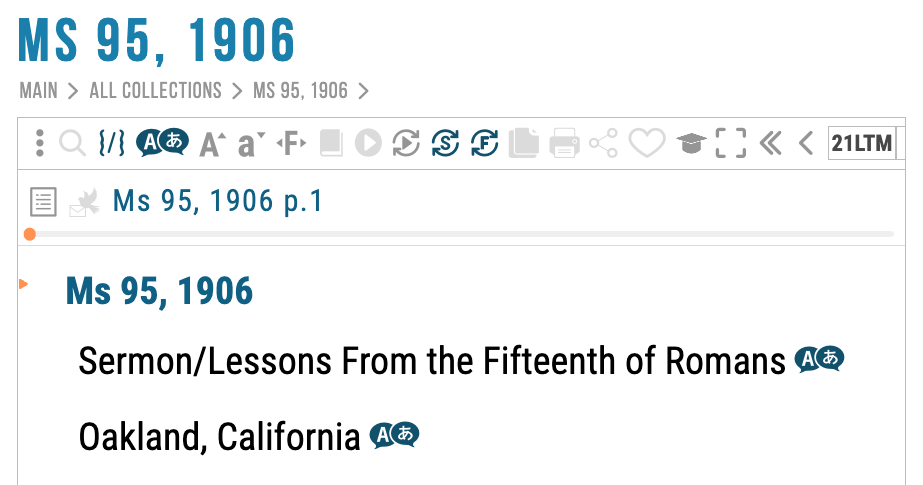
\includegraphics[width=1\linewidth]{images/sermons-and-talks.png}
    \label{fig:enter-label}
\end{figure}

For us, personally, these quotations are unauthenticated and, especially, invalid compared to Ellen White’s authenticated works. But if someone insists on weighing her unconfirmed reports and published writings equally, we will not stand in their way but even further push the conclusion of the Holy Spirit as a being. Let’s follow together.

Even compared with Ellen White’s authenticated works, such a Holy Spirit, a being, would not be one with God because Christ was \egwinline{\textbf{The only being who was one with God}}[Lt121-1897.7; 1897][https://egwwritings.org/read?panels=p7266.13]. This Holy Spirit, a being, could not \egwinline{\textbf{enter into all the counsels and purposes of God}}, because Christ was \egwinline{\textbf{the only being}}[PP 34.1; 1890][https://egwwritings.org/read?panels=p84.75] who could do that. This Being is not to be exalted because \egwinline{\textbf{The Father and the Son \underline{alone} are to be exalted}}[YI, July 7, 1898 par.2.; 1898][https://egwwritings.org/read?panels=p469.2964]. The Holy Spirit, as a being, would not fit in the order of heaven as the third being because Satan was \egwinline{\textbf{next to Christ the most exalted \underline{being}} in the heavenly courts}[RH August 9, 1898, par. 7; 1898][https://egwwritings.org/read?panels=p821.17145]. This Holy Spirit, a being, was not invested in the cost of salvation; neither was he in the covenant with Father and Son to save the world, nor dishonored by man’s transgression.

\egwinline{The great gift of salvation has been placed within our reach at an \textbf{infinite cost to the Father and the Son}.}[RH November 21, 1912, par. 2; 1912][https://egwwritings.org/read?panels=p821.33329]

\egwinline{In the plan to save a lost world, the counsel was between them \textbf{\underline{both}}; \textbf{the covenant of peace was between the Father and the Son}.}[ST December 23, 1897, par. 2; 1897][https://egwwritings.org/read?panels=p820.14803]

\egwinline{But in the transgression of man \textbf{\underline{both} the Father and the Son were dishonored}.}[ST December 12, 1895, par. 7; 1895][https://egwwritings.org/read?panels=p820.13243]

Such a Holy Spirit, a being, does not fit into harmony with the authenticated reports of Ellen White, nor with the Scriptures. The Holy Spirit is called ‘\textit{spirit}’, so it is a spirit, exclusively.

Many of Sister White’s quotations are sourced from sermons or talks that were published after her death. In what follows, we will present a few that are most often discussed in an effort to prove that Sister White was a trinitarian. We invite everyone to weigh these quotations with her authenticated and published work, those during her lifetime.

“\textit{And then the golden harps are touched, and the music flows all through the heavenly host, and they fall down and worship the Father and the Son and the Holy Spirit}.”\footnote{\href{https://egwwritings.org/?ref=en_Ms139-1906.32&para=9579.38}{EGW; Ms139-1906.32; 1906}} [Sermon/Thoughts on Matthew 4. Oakland, California July 24, 1906; Previously unpublished.]

“\textit{We need to realize that the Holy Spirit, who is as much a person as God is a person, is walking through these grounds.}”\footnote{\href{https://egwwritings.org/?ref=en_Ms66-1899.11&para=6622.19}{EGW; Ms66-1899.11: 1899}} [Talk/Extracts From Talks Given by Mrs. E. G. White at the Opening of College Hall, Avondale, and in the Avondale Church]